\section{Methodology}\label{sec:Methodology}

In this section, our goal is to build an in-depth understanding of the network traffic generated by apps at the network access point, and investigate how this traffic can improve the performance of the \mas for detection of malicious apps. To achieve this goal, we investigate the following research questions:

\begin{enumerate}[(RQ1)]
\item \rqa
\item \rqb
\item \rqc
% \review{\item \rqe}
\end{enumerate}

In rest of the section, we discuss our study settings as follows. First, we present how we curated an Android repackaged apps dataset that spanned a diverse range of malware families (Section~\ref{sec:dataset}). Second, we presented how \mas collect data from sensitive APIS calls, from original and repackaged apps, and how our platform also extracted network traffic generated by these apps at the network access point (Section~\ref{sec:mas}) and (Section~\ref{sec:traffic}).  Then, we explain how we collected features from this traffic (Section~\ref{sec:extraction}). Finally, we described the procedures we used to detect malicious behaviors in repackaged apps based on machine learning and how we interpreted the results (Section~\ref{sec:learning}) and (Section~\ref{sec:understand}).

\subsection{Malware Dataset}\label{sec:dataset}


To test and evaluate our proposal, we used the same dataset built by the \fhc. The dataset (hereafter referred to as \cds) contains 4,076 real-world app pairs from three repackaged app repositories (\repack~\cite{DBLP:journals/tse/LiBK21}, \amc~\cite{rafiq2022andromalpack} and Androzoo repository~\cite{DBLP:conf/msr/AllixBKT16}), along with their respective original apps. Of these, $1,777$ are original versions, and $4,076$ are repackaged versions—multiple repackaged versions of the same original app may coexist within the \cds dataset.

To ensure that all original apps were not malware, the authors queried the \vt repository, confirming that no antivirus engines flagged them as malicious. \vt is a popular tool used by researchers and practitioners to check software assets, including Android apps, using more than 60 security engines~\cite{DBLP:journals/ese/KhanmohammadiEH19}. The authors also evaluated the repackaged versions with \vt and confirmed that $71.02$\% of the repackaged apps were malicious (2,895 out of the 4,076 repackaged apps).

The \cds contains information about malware families, the similarity between the original and repackaged app versions, and the source of the Android app store. The app store source information was obtained from the three original repackaged app repositories, while the other features were extracted using the \avt~\cite{avclass2-paper} (for malware family identification) and the SimiDroid tool~\cite{DBLP:conf/trustcom/0029BK17} (for similarity scoring). According to the \fhc, the \cds comprises 116 distinct malware families, most of them from the \gps family ($46.18$\%), and an average similarity score of $90.39$\%, with the majority of app pairs ($3,587$) having more than 75\% similarity. Regarding the Android app store source, most of the repackaged apps come from the non-official Android app store, Anzhi~\cite{anzhi}.



\subsection{\mas Data Collection Procedure}\label{sec:mas}


To collect sensitive data from all apps, the \fhc leverages the DroidXP infrastructure~\cite{DBLP:conf/scam/CostaMCMVBC20}. As demonstrated in the study, DroidXP can compare test case generation tools in terms of identifying malicious app behaviors using the \mas, making it a valuable tool for automating the following steps:


\begin{enumerate}[1.]
 \item \textbf{Instrumentation}: As a first step, the \fhc uses DroidXP to instrument all pairs of apps in the \cds. Both versions of the apps are instrumented to collect relevant information during their execution. In the background, DroidXP leverages DroidFax to gather static information about all apps (both original and repackaged versions). As noted by the authors, to improve performance across multiple executions, this phase is performed only once for each version of the apps in the \cds


\item \textbf{Execution}: DroidXP then installs the instrumented version of the apps on an Android emulator. As statistical result show that $83.8\%$ of malware are activity after restart~\cite{DBLP:conf/sp/ZhouJ12}, the author report that restart the installed app, before the effective execution. Then, they initiate a test case generation tool (DroidBot~\cite{DBLP:conf/icse/LiYGC17}) to execute both versions of the app. The authors justify the use of DroidBot by citing a previous research~\cite{DBLP:conf/wcre/BaoLL18} that reports higher accuracy in sandboxes built, using the \mas combined with DroidBot as the test case generation tool. They also report that this same research indicates DroidBot’s coverage reaches near-maximum within one minute. For this reason, each app is run for one minute, and three times, to mitigate the randomness involved in test case generation tools.

\item \textbf{Data Collection}: At the end of the execution step, the \fhc once again leverages DroidFax through DroidXP, this time to collect all relevant information, such as calls to sensitive APIs. This data is then used to analyze the performance of the \mas in detecting malicious behavior.
\end{enumerate}



The study consider that a sandbox of app identifies a malware whenever the malicious app version makes a call to a sensitive API, which was not called during the exploratory phase of your original version, as present at Figure~\ref{fig:mine}.


\begin{figure*}[h]
  \centering
  
    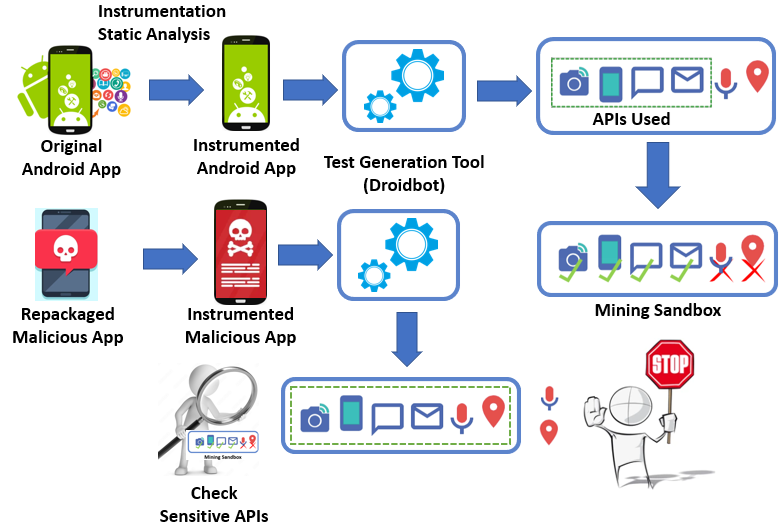
\includegraphics[width=0.55\textwidth]{image/mineSandbox.png} \\[\abovecaptionskip]
    
  \caption{Overview of \fhc for malware identification}\label{fig:mine}
\end{figure*}


\subsection{Traffic Collection Procedure}\label{sec:traffic}

To extract traffic data generated by both malicious and benign apps (4,076 app pairs), we also utilize DroidXP, which uses the TcpDump tool to collect inbound and outbound network traffic. As described in section 3.2, in the second step of our study (Execution), DroidXP also collects all packet capture (PCAP) files~\cite{DBLP:conf/iv/UhlarHR21} of all explored apps (1,182 original and 2,894 malicious). A PCAP file contains copies of trafficked packets over the network, allowing analysis of all values of payloads and packet headers~\cite{DBLP:conf/iv/UhlarHR21}. Because storing and processing PCAP files is very expensive, it is necessary to perform just a limited network segment analysis, rather than analyzing all of them. To extract the most relevant features for our study from all generated PCAP files, we utilize CICflowMeter~\cite{DBLP:conf/icissp/LashkariDMG17}, as we describe in the next section.

\subsection{Feature Extraction}\label{sec:extraction}

To extract features, we processed each traffic file (PCAP file) generated by DroidXP at explored step, creating features sets in the format of CSV files, for respective PCAP file. In the end, we combine all CSV files in just one, with total of 86 features, which we will not describe here, because of limited space. We do not considered all of them, and removed some features that were made up within at our simulated environment or do not make sense for our study like: Flow ID, Source IP, Destination IP, Source Port, Source MAC, Destination MAC, Protocol and Timestamp. In the end, we remain with 78 features.

Secondly, we filtered our CSV file by the feature "Destination Port." We used only the 15 most relevant Destination Ports, which are the ones that appear most frequently in our CSV file. (see Table~\ref{tab:port}).

\begin{table}[h]
  \caption{THE 15 MOST RELEVANT DESTINATION PORT.}
  \centering
  \begin{small}
    \begin{tabular}{rrlr}   \hline
 \# & Port & Description & Occurs  \\ \hline

1 &  443 &  Hypertext Transf. Protocol Secure &  1275293  \\ 
  2 &  53 & Domain Name System & 641965  \\ 
  3 &  80 & Hypertext Transfer Protocol &  38830  \\ 
  4 &  853 & DNS over TLS &  32784  \\ 
  5 &  5228 & Google Cloud Messaging &  26509  \\ 
  6 &  123 & Network Time Protocol & 9179  \\ 
  7 &  68 & Dynamic Host Config. Protocol &  8091  \\ 
  8 &  67 & Dynamic Host Config. Protocol &  8091  \\ 
  9 &  9999 & HyperSQL Database &  268  \\ 
  10 & 8080 & Hypertext Transfer Protocol & 221  \\ 
  11 & 6881 & BitTorrent Protocol & 173  \\ 
  12 & 5566 & Network Monitoring & 110  \\ 
  13 & 8881 & Hypertext Transfer Protocol & 110  \\ 
  14 & 9002 & Management Interfaces & 106  \\ 
  15 & 7 & Echo Protocol & 84  \\ 
   \hline

 \end{tabular}
 \end{small}
 \label{tab:port}
 \end{table}


\begin{table}[ht]
  \caption{STATISTICAL FUNCTIONS AT FEATURES.}
  \centering
  \begin{small}
    \begin{tabular}{rllrr}   \hline
 \# & Function & Description\\ \hline

1 &  min &  Minimum\\ 
  2 &  max & Maximum\\ 
  3 &  sum & Amount\\ 
  4 &  mean & Average\\ 
  5 &  std & Standard deviation \\ 
  6 &  median & Median\\ 
  7 &  count & Number of observation\\ 
  8 &  var & Variance\\ 
  9 &  skew & Skewness \\ 
   \hline

 \end{tabular}
 \end{small}
 \label{tab:function}
 \end{table}


\subsubsection{Flow features set}\label{sec:set}

The next step in formatting our flow feature set involves the combination of the initial 76 features (excluding Destination Port and Hash), 15 Destination Ports, and 9 statistical functions listed in Table~\ref{tab:function}. This combination greatly enhances the convenience of our experiment when we use it with machine learning algorithms to train detection models. By the end of this step, we have a dataset with a total of 10,262 features ($76\times15\times9$) + Hash + Type (benign/malicious).

However, according to the literature~\cite{DBLP:conf/ichmi/Xie22,DBLP:journals/mta/AmiriebrahimabadiM24}, selecting relevant features is crucial for achieving good predictive power in a machine learning model. This can improve model accuracy and reduce training time, especially in high-dimensional datasets. With this objective, we selected the most relevant features based on the model used in our research, the Random Forest~\cite{james2023introduction}, which we discuss at Section~\ref{sec:learning}. To achieve greater efficiency from the Random Forest model, we selected the 20 most relevant features based on Gini Importance or Mean Decrease in Impurity (MDI)~\cite{james2023introduction}. The final selected features used in our research are listed at Table~\ref{tab:features}.

\begin{table*}[ht]
  \caption{THE 20 MOST RELEVANT FEATURES.}
  \centering
  \begin{small}
    \begin{tabular}{rrlrrr}   \hline
 \# & Feature & Description & Function & Port & Importance  \\ \hline

1 &  \texttt{bwd\char`_byts\char`_b\char`_avg} &  Average bytes per bulk in the backward direction &  max & 443& 0.1737\\ 
  2 &  \texttt{bwd\char`_byts\char`_b\char`_avg} &Average bytes per bulk in the backward direction & median & 443& 0.0911\\ 
  3 &  \texttt{bwd\char`_byts\char`_b\char`_avg} & Average bytes per bulk in the backward direction &  max  & 5228& 0.0467\\ 
  4 &  \texttt{fwd\char`_pkt\char`_len\char`_min} &Minimum length of packet in the fwd. dir. &  sum  & 443&0.0239\\ 
  5 &  \texttt{init\char`_fwd\char`_win\char`_byts} & Num. of bytes in the initial window in the fwd dir. &  sum  & 853&0.0200\\ 
  6 &  \texttt{pkt\char`_len\char`_mean} & Mean length of a packet & median  & 443& 0.0185\\ 
  7 &  \texttt{pkt\char`_size\char`_avg} &Average size of the packet &  median  & 443&0.0183\\ 
  8 &  \texttt{fwd\char`_blk\char`_rate\char`_avg} & Average rate of bulk in the forward direction &  sum  & 443&0.0164\\ 
  9 &  \texttt{subflow\char`_bwd\char`_byts} & Number of bytes in a subflow in the backward dir. &  max  & 443&0.0160\\ 
  10 & \texttt{init\char`_fwd\char`_win\char`_byts} & Num. of bytes in the initial win. in the fwd. dir. & sum  & 443&0.0141\\ 
  11 & \texttt{totlen\char`_bwd\char`_pkts} & Total length of packets in the bck. dir. & max  & 443 &0.0130\\ 
  12 & \texttt{flow\char`_duration} & Duration of the flow in microseconds & sum  & 123 &0.0118\\ 
  13 & \texttt{bwd\char`_pkt\char`_len\char`_max} & Maximum length of packet in the bck. dir. & sum  & 443&0.0112\\ 
  14 & \texttt{pkt\char`_len\char`_max} & Maximum length of a packet & sum  & 443&0.0112\\ 
  15 & \texttt{fwd\char`_seg\char`_size\char`_min} & Minimum segment size observed in the fwd. dir. & sum  & 443&0.0100\\ 
  16 & \texttt{flow\char`_byts\char`_s} & Flow rate in bytes per second & sum  & 80&0.0084\\ 
  17 & \texttt{bwd\char`_pkt\char`_len\char`_mean} & Mean length of packets in the backward dir. & max  & 443&0.0081\\ 
  18 & \texttt{bwd\char`_seg\char`_size\char`_avg} & Average size of the segment in the backward dir. & max  & 5228&0.0078\\ 
  19 & \texttt{pkt\char`_len\char`_mean} & Mean length of a packet & max  & 5228&0.0073\\ 
  20 & \texttt{pkt\char`_size\char`_avg} & Average size of the packet & max  & 5228 &0.0072\\ 
   \hline

 \end{tabular}
 \end{small}
 \label{tab:features}
 \end{table*}

\subsection{Learning-based Detection Procedures}\label{sec:learning}

Machine learning techniques are used to automate the rule discovery process through data analysis, enabling the prediction of unknown data. In our experiment, we use machine learning to perform flow-based classification by analyzing their properties such as source/destination port, number of packets, and flow duration.

To find the best network flow classification and training method, we first investigated four popular approaches: Linear Discriminant Analysis (LDA), Quadratic Discriminant Analysis (QDA), Logistic Regression, and the Random Forest algorithm~\cite{james2023introduction}. Subsequently, we explored a novel classifier called Energy-Based Flow Classifier (EFC), which is inspired by the inverse Potts model from quantum mechanics~\cite{DBLP:journals/tnsm/PontesSGBM21}. Among these methods, the supervised approach Random Forest delivered the best performance. This algorithm aggregates multiple decision trees, with each tree constructed using a random subset of features. The process decorrelates the trees, allowing for a more thorough exploration of the model and substantially improving predictive performance~\cite{james2023introduction}.

In our learning-based detection procedure, we split the feature set into a training set consisting of $70$\% of the samples and a testing set consisting of $30$\%, randomly selected from the \cds. The testing set is used solely to evaluate the detection accuracy of the procedure. To achieve the best-fitting model, we varied several model parameters using cross-validation~\cite{DBLP:phd/us/Stephenson22} on the training data. Cross-validation is a technique used in machine learning to assess how well a model performs on an independent dataset~\cite{DBLP:journals/jsan/AwadF23}. The technique tests the model on different parts of the data, helping detect overfitting, making efficient use of the available data. For our experiment, it selected a model with 7 parameters, including:

\begin{itemize}
    \item Number of trees in the forest: $400$
    \item The minimum number of samples required to split an internal node: $18$
    \item The minimum number of samples required to be at a leaf node: $3$
    \item The number of features to consider when looking for the best split: $\log_2(features)$
    \item The maximum depth of the tree: None~\footnote{If None, then nodes are expanded until all leaves}
\end{itemize}

\subsection{Understanding Results}\label{sec:understand}

To understand our results, we divide our result into two steps. First, we present the results of \fhc, which report the effectiveness of \mas using DroidBot as test generation tool for sandbox construction. The study labels a repackaged version of an app as malware if there is at least one call to a sensitive API that (a) was observed while executing the repackaged version of the app and (b) was not observed while executing the original version of the same app. If the set of sensitive methods called only by the repackaged version of an app is empty,  \fhc conclude that the sandbox does not label the repackaged app as malware.

In the next step, we began our study, using machine learning (ML) technique, which involved training the model, base on flow properties, and later using it for malware classification. The result of the \ml provides predictions for all samples according to the trained model. Finally, we triangulate the results of the \mas classification, coming from \fhc, and our \ml classification, with the outputs of \vt, which may lead to one of the following situations:

\begin{itemize}
\item {\bf True Positive (TP)}. The \mas or \ml label a repackaged version as a malware and, according to
  \vt, at least two \ses label the asset as a malware. This decision aligns with existing recommendations~\cite{vt-label,DBLP:journals/ese/KhanmohammadiEH19}
   
\item {\bf False Positive (FP)}. The \mas or \ml label a repackaged version as a malware and, according to \vt, at most one \se labels the asset as a malware.

\item {\bf False Negative (FN)}. The \mas and \ml does not label a repackaged version as a malware, and according to \vt, at least two \ses label the asset as a malware.
\end{itemize}

We compute \emph{Precision}, \emph{Recall}, and \emph{F-measure} ($F_1$) from
the number of true-positives, false-positives, and false-negatives (using standard
formulae). We use basic statistics (average, median, standard deviation) to identify the
accuracy of the \mas and \ml for malware classification, at our \cds.



